The aim of this chapter is to test and analyze projects from git by using developed module for RefactorErl. The projects selected for the experiment are written in Erlang and have more than 40 commits.

\section{Iron}

This project is functional Erlang Toolkit. Iron is released under the MIT license. It can do the foolowing:
\begin{itemize}
	\item Count with coerce equality, count with custom predicate.
	\item Find with coerce equality, find with custom predicate.
\end{itemize}

This project has just only one source code file with 68 commits. The link to the ripository is \url{https://github.com/elementerl/iron}

We can see that with the version number increase the line of code number and char of code number also grow on Figure \ref{fig:loc_iron} and on Figure \ref{fig:char_iron}.

\begin{figure}[h]
	\centering
	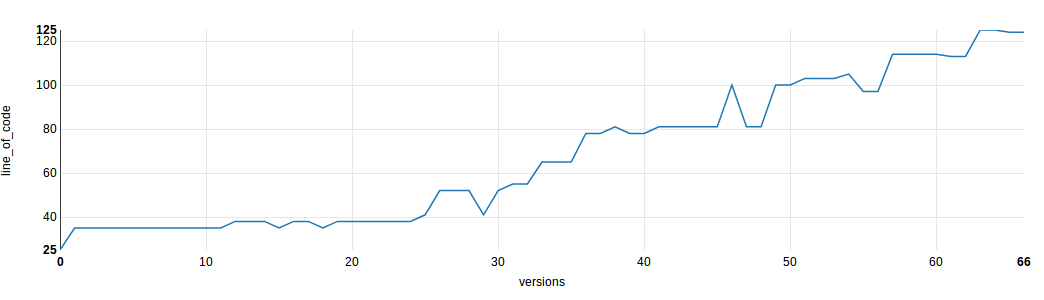
\includegraphics[height=45mm]{figures/loc_iron.png}
	\caption{Effective Line of code for fe.erl file.}
	\label{fig:loc_iron}
\end{figure}

\begin{figure}[h]
	\centering
	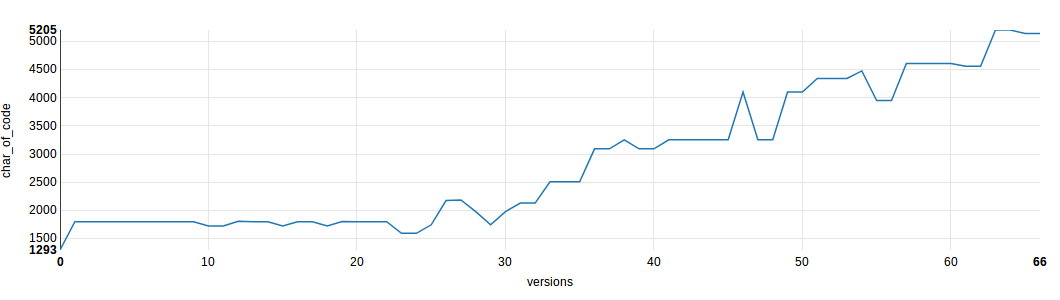
\includegraphics[height=45mm]{figures/char_iron.png}
	\caption{Char of code for fe.erl file.}
	\label{fig:char_iron}
\end{figure}

As shown on Figure \ref{fig:otp_iron} developer started to use otp library after 45th version. 

\begin{figure}[h]
	\centering
	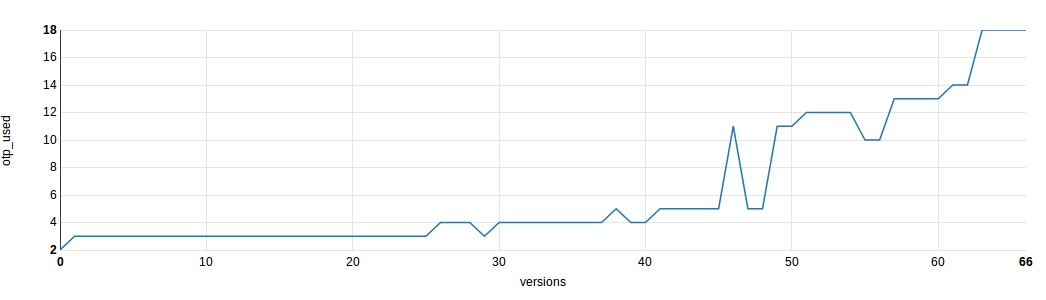
\includegraphics[height=45mm]{figures/otp_iron.png}
	\caption{Otp used for fe.erl file.}
	\label{fig:otp_iron}
\end{figure}

Average length of line was not stabilize until arround 35th version with gradually decreasing from 50 symbols to 38 symbols.

\begin{figure}[h]
	\centering
	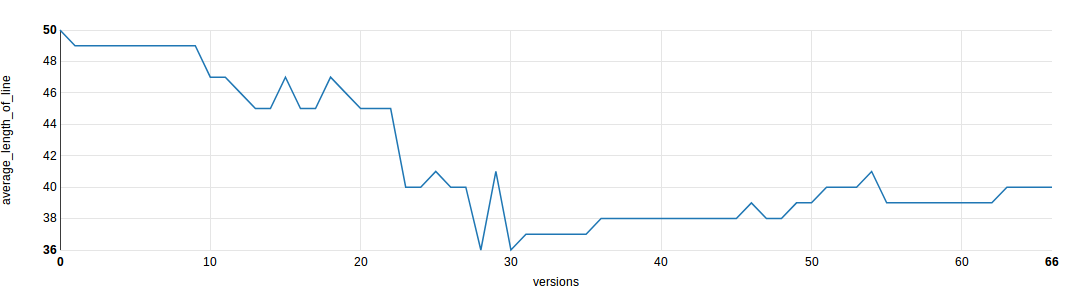
\includegraphics[height=45mm]{figures/average_length_of_line_iron.png}
	\caption{Average length of line for fe.erl file.}
	\label{fig:average_length_of_line_iron}
\end{figure}

As we can see on Figure \ref{fig:number_of_macros_iron} and Figure \ref{fig:number_of_records_iron} there are not defined macros and record in the whole iron project.

\begin{figure}[h]
	\centering
	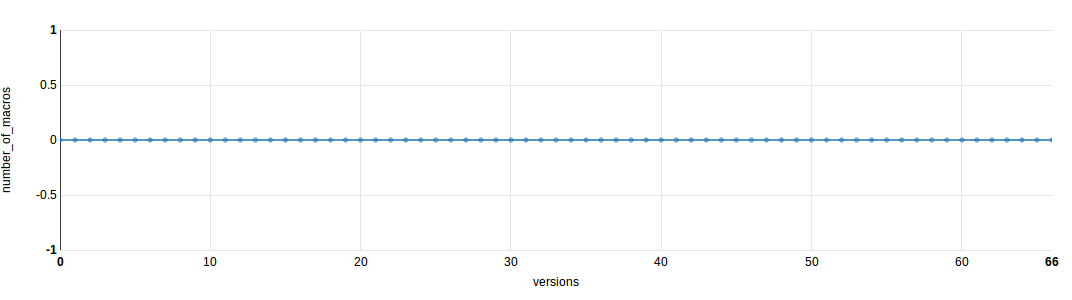
\includegraphics[height=45mm]{figures/number_of_macros_iron.png}
	\caption{Number of macros for fe.erl file.}
	\label{fig:number_of_macros_iron}
\end{figure}

\begin{figure}[h]
	\centering
	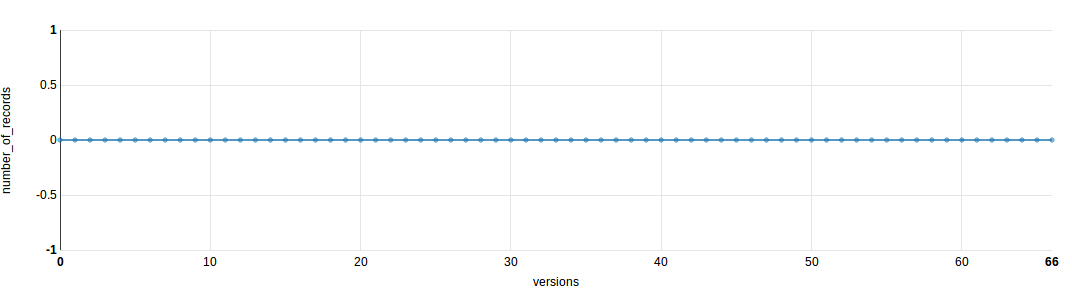
\includegraphics[height=45mm]{figures/number_of_records_iron.png}
	\caption{Number of records for fe.erl file.}
	\label{fig:number_of_records_iron}
\end{figure}

\section{Erlang chat }

This project is multi user chat written in Erlang. It has nine source code files and 45 commits. The link to the ripository is \url{https://github.com/bildeyko/erlangChat}

For this project we analyzed the module websocket\_handler.erl. This module consists 6 functions.

The Figure \ref{fig:loc_chat} shows the changing of number of lines of code.

\begin{figure}[h]
	\centering
	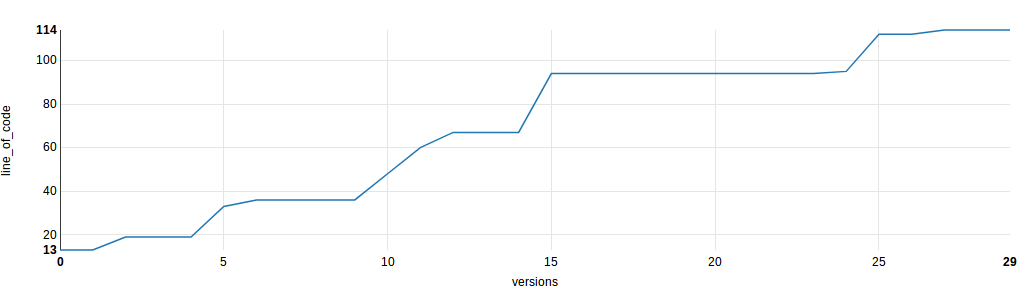
\includegraphics[height=45mm]{figures/loc_chat.png}
	\caption{Effective Line of code for websocket\_handler.erl.}
	\label{fig:loc_chat}
\end{figure}

In the Figure \ref{fig:chat} we can see that the author started using message passing from the 9th version of his software.

\begin{figure}[h]
	\centering
	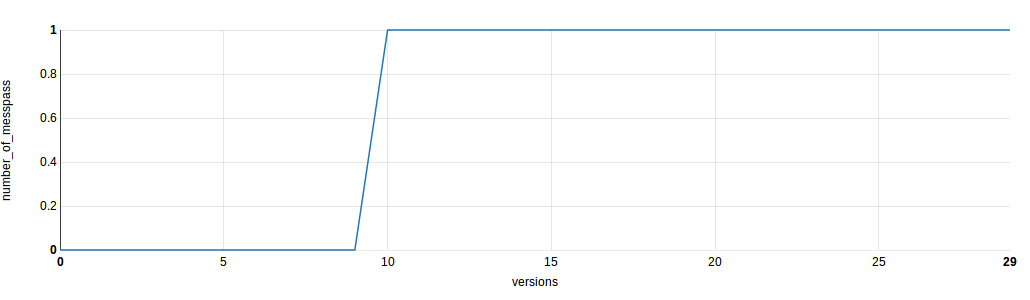
\includegraphics[height=45mm]{figures/chat.png}
	\caption{Number of message passing for websocket\_handler.erl.}
	\label{fig:chat}
\end{figure}

As shown in Figure \ref{fig:chat5} there was incresing length of the longest line of code in 9th version. 
\begin{figure}[h]
	\centering
	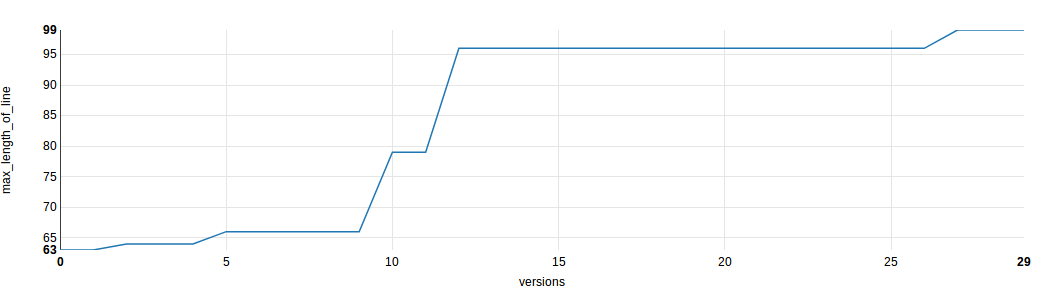
\includegraphics[height=45mm]{figures/chat5.png}
	\caption{Max length of line for websocket\_handler.erl.}
	\label{fig:chat5}
\end{figure}

Measurement of McCabe’s cyclomatic complexity metric ensures that developers are sensitive to the fact that programs with high McCabe numbers (e.g. > 10) are likely to be difficult to understand and therefore have a higher probability of containing defects. The tested module has the cyclomatic complexity number which increased to 3o in last versions as shown in Figure \ref{fig:mcCabe}.

\begin{figure}[h]
	\centering
	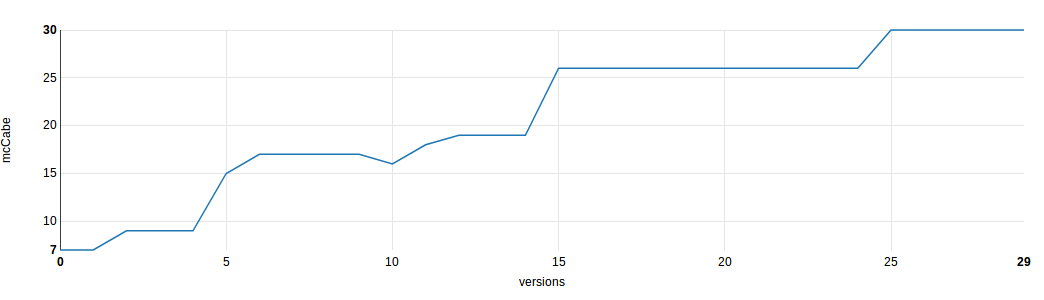
\includegraphics[height=45mm]{figures/mcCabe.png}
	\caption{
	McCabe cyclomatic complexity metric for websocket\_handler.erl.}
	\label{fig:mcCabe}
\end{figure}

In Figure \ref{fig:chat2} shows that developer used otp library functions but after 9th version reconsidered to use them.

\begin{figure}[h]
	\centering
	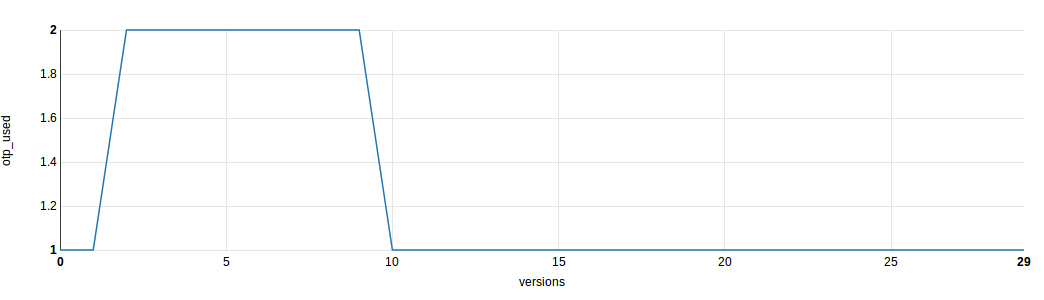
\includegraphics[height=45mm]{figures/chat2.png}
	\caption{
		Otp used for websocket\_handler.erl.}
	\label{fig:chat2}
\end{figure}

The developed framework allows to measure and visualayze metrics for module and also for each function in the module. For example, in this module developer use message passing from 9th version as we mensioned above. The Figure \ref{fig:chat3} shows that there was discovered function in which author actively used message passing.

\begin{figure}[h]
	\centering
	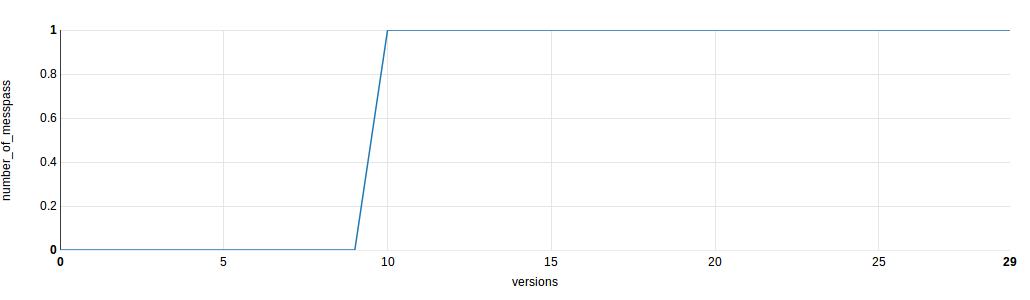
\includegraphics[height=45mm]{figures/chat3.png}
	\caption{
	Number of message passing for function websocket\_handle/3.}
	\label{fig:chat3}
\end{figure}

Visualyzing of metrics helps to find which functions have been changed, added or deleted. As shown in the Figure\ref{fig:chat3} the developer slightly changed the function terminate/3 by adding two lines of code in 9th version.
\begin{figure}[h]
	\centering
	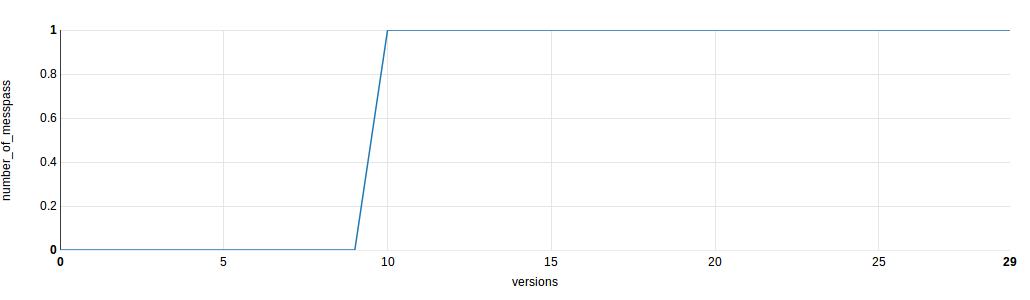
\includegraphics[height=45mm]{figures/chat3.png}
	\caption{
		Number of message passing for function websocket\_handle/3.}
	\label{fig:chat3}
\end{figure}
 
To summarize findings we can assume that most of these changes was done in 9th version.

\section{prx}

This project is an Erlang library for Unix process management and system programming tasks. Code from all project is divided into 4 modules. 

The project provides:

\begin{itemize}
	\item Beam-friendly interface to system calls and other POSIX operation.
	\item Reliable OS process management by mapping Erlang processes to a hierarchy of system processes.
	\item An interface for privilege separation operations to restrict processes.
	\item Operations to isolate processes like containers and jails.
\end{itemize}


The link to the ripository is\url{https://github.com/msantos/prx}. This project has 201 commits. 



